
As the line at the direction of (1  2  -1$)^T$ is represented by $\vec{b}$, so $\vec{b}$ is the direction vector and the point is $\vec{a}$ = (2  -1  4$)^T$ through which the line passes through.\\
From the problem statement, we got

\begin{align}
\vec{a} = \begin{pmatrix}
      2 \\ 
      -1 \\
      4 \\
      \end{pmatrix} 
\end{align}

So, let us consider another point $P$ with $\vec{r}$ = (x y z$)^T$ on the line that passes through $\vec{a}$. \\

\begin{align}
\vec{r} = \vec{a} + \lambda \vec{b} 
\end{align}

 Fig. \ref{fig:solutions/line_plane/68point_distance}

\begin{figure}[!ht]
\centering
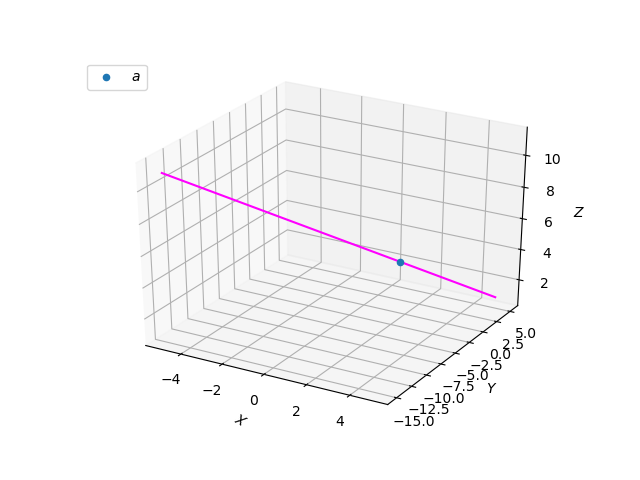
\includegraphics[width=\columnwidth]{./solutions/line_plane/68/figs/line_Eqn3.png}
\caption{The Straight line passing through a point at a particular direction}
\label{fig:solutions/line_plane/68point_distance}
\end{figure}

